% Where the collocation points actually sit, for K = 3 and K = 5, in all three
% Gauss-Jacobi families. Authored 2026-09-14 in answer to Alex's note after
% teaching Lecture 7:
%
%     "Page 7-8. It is not clear how alpha and beta connect into any specific
%      formula. It would be a lot more helpful to show a sketch comparing the
%      collocation points for K=3 and K=5 for these three methods."
%
% and, for the second use of the same picture:
%
%     "Page 7-10. The point about Radau and Lobatto versus Legendre for
%      connectivity is hard to understand. In Page 7-8, I suggested adding a
%      picture. It would be good to have the same (or similar) picture here."
%
% THE POINT OF THE FIGURE, in one line: alpha and beta are the exponents of the
% Jacobi weight, and setting one of them to 1 PINS the corresponding endpoint as
% a collocation point -- beta pins tau = 0, alpha pins tau = 1. Read down the
% figure and the three families are one family with 0, 1 or 2 endpoints pinned.
% That also explains the truncation-error column on the same handout page: an
% n-point rule with no pinned node is exact to degree 2n-1 (O(h^2K)); each
% pinned node is one fewer FREE node, so the order drops by exactly one --
% O(h^2K-1) for Radau, O(h^2K-2) for Lobatto. The two columns of that table are
% the same fact seen twice.
%
% PROVENANCE OF THE NUMBERS. 🔴 Read this before "correcting" any value.
%   * Legendre and Radau are Biegler, Table 10.1, printed p. 292, transcribed
%     from the book and independently recomputed (numpy, shifted Legendre roots
%     and the right-Radau construction) -- both agree to all six printed digits.
%     K=3 Radau also appears worked in Biegler's own Example 10.2, p. 294.
%   * LOBATTO IS NOT IN TABLE 10.1. Biegler tabulates only Legendre and Radau
%     ("We will focus on Gauss-Legendre and Radau collocation", p. 292). The
%     Lobatto values here are DERIVED: endpoints plus the roots of P'_{K-1}
%     shifted to [0,1], i.e. 0, 1/2, 1 for K=3 and 0, 0.172673, 1/2, 0.827327, 1
%     for K=5. Marked \authored in the lecture for that reason.
%   * RADAU HERE IS RIGHT-RADAU (Radau IIA), the course's choice, so tau_K = 1.
%     The left-Radau family pins tau = 0 instead and is the mirror image; the
%     lecture says which one it uses at Sec. IX. Do not "fix" the asymmetry.
%
% GREYSCALE. Two hues, Okabe-Ito blue #0072B2 (L* 46) and orange #E69F00
% (L* 70.6). Nothing is carried by colour alone: K=3 is FILLED CIRCLES above the
% axis, K=5 is OPEN SQUARES below it, so the two series are separated by shape
% and by side as well as hue. The pinned endpoints carry a heavy vertical rule
% spanning all three rows, which is the comparison the figure exists to make.
%
% TIKZ LIBRARIES. Base tikz only, plus the >=stealth arrow tip.

% LAYOUT NOTE, 2026-09-14. The family name and the (alpha, beta) pair live in a
% LEFT GUTTER at negative x, not on the axis. First draft put them at the axis
% origin: the tau = 0 rule then struck through the "G" of each name and the
% (alpha, beta) text ran underneath the K=5 squares. Found by rendering the page
% at 130 dpi and looking at it -- it compiled cleanly both times, so no checker
% would have caught either collision.
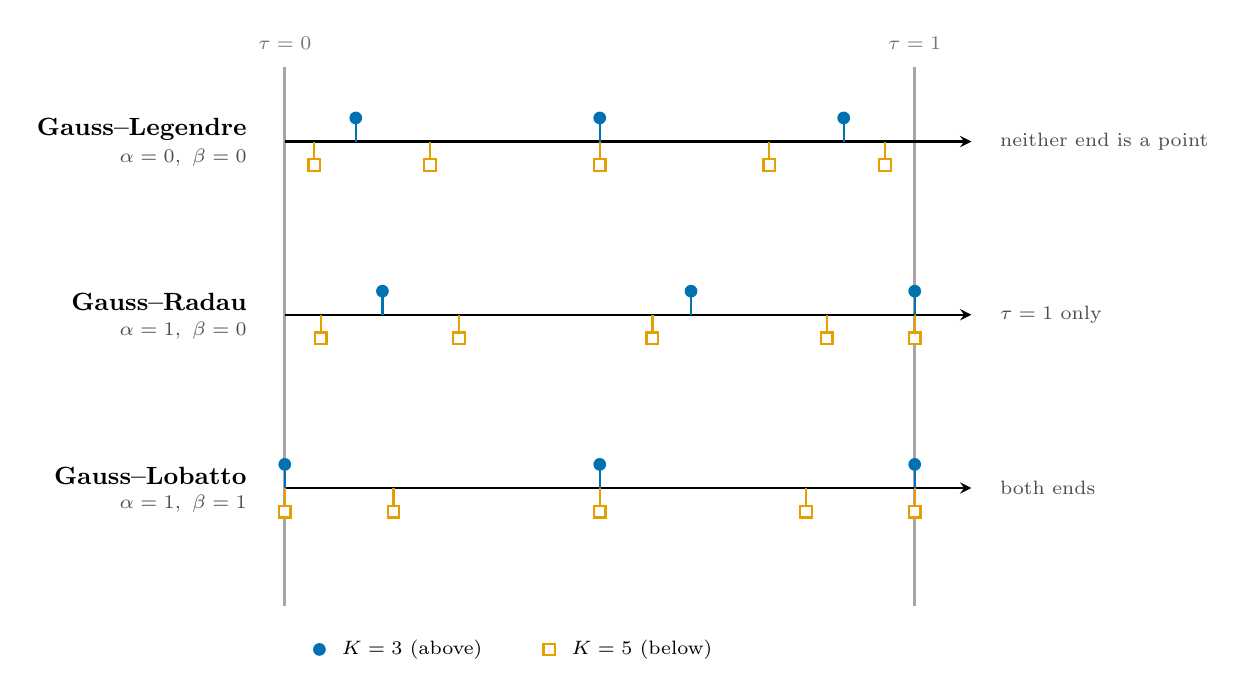
\begin{tikzpicture}[x=8cm, y=1cm, >=stealth]
  \definecolor{cpblue}{HTML}{0072B2}
  \definecolor{cporange}{HTML}{E69F00}

  % ---- the two endpoint rules, drawn first so the axes sit on top ----------
  \draw[black!35, line width=1.1pt] (0,0.95) -- (0,-5.9);
  \draw[black!35, line width=1.1pt] (1,0.95) -- (1,-5.9);
  \node[black!55, font=\scriptsize] at (0,1.25) {$\tau=0$};
  \node[black!55, font=\scriptsize] at (1,1.25) {$\tau=1$};

  % ---- one row per family --------------------------------------------------
  % #1 y offset, #2 family name, #3 (alpha,beta), #4 K=3 list, #5 K=5 list,
  % #6 the endpoint verdict
  \foreach \yy/\fam/\ab/\three/\five/\verdict in {%
    0/{Gauss--Legendre}/{$\alpha=0,\ \beta=0$}/{0.112702,0.5,0.887298}/%
      {0.046910,0.230765,0.5,0.769235,0.953090}/{neither end is a point},
    -2.2/{Gauss--Radau}/{$\alpha=1,\ \beta=0$}/{0.155051,0.644949,1}/%
      {0.057104,0.276843,0.583590,0.860240,1}/{$\tau=1$ only},
    -4.4/{Gauss--Lobatto}/{$\alpha=1,\ \beta=1$}/{0,0.5,1}/%
      {0,0.172673,0.5,0.827327,1}/{both ends}%
  }{
    % axis
    \draw[->, thick] (0,\yy) -- (1.09,\yy);
    % family label + Jacobi parameters, in the LEFT GUTTER (see layout note)
    \node[anchor=east, font=\small\bfseries] at (-0.045,\yy+0.16) {\fam};
    \node[anchor=east, font=\scriptsize, black!70] at (-0.045,\yy-0.20) {\ab};
    % K = 3, filled circles ABOVE the axis
    \foreach \t in \three {
      \draw[cpblue, thick] (\t,\yy) -- (\t,\yy+0.30);
      \fill[cpblue] (\t,\yy+0.30) circle (2.3pt);
    }
    % K = 5, open squares BELOW the axis
    \foreach \t in \five {
      \draw[cporange, thick] (\t,\yy) -- (\t,\yy-0.30);
      \draw[cporange, thick, fill=white]
        (\t,\yy-0.30) +(-2.1pt,-2.1pt) rectangle +(2.1pt,2.1pt);
    }
    % verdict
    \node[anchor=west, font=\scriptsize, black!70] at (1.12,\yy) {\verdict};
  }

  % ---- legend --------------------------------------------------------------
  \fill[cpblue] (0.055,-6.45) circle (2.3pt);
  \node[anchor=west, font=\scriptsize] at (0.075,-6.45) {$K=3$ (above)};
  \draw[cporange, thick, fill=white]
    (0.42,-6.45) +(-2.1pt,-2.1pt) rectangle +(2.1pt,2.1pt);
  \node[anchor=west, font=\scriptsize] at (0.44,-6.45) {$K=5$ (below)};
\end{tikzpicture}
